\documentclass[12pt, letterpaper]{article} 
 \usepackage{graphicx} 
 \usepackage{hyperref} 
 \usepackage[utf8]{inputenc} 
 \usepackage{float} 
 \usepackage{geometry} 
 \usepackage{enumitem, array} 
 \usepackage{longtable} 
 \usepackage{lscape} 
 \usepackage[export]{adjustbox} 
 \geometry{letterpaper,left=10mm,right=10mm,bottom=20mm,top=20mm} 
 \graphicspath{ {./../img/simulation/} } 
 \renewcommand{\rule}{Regla 22} 
 \renewcommand{\r}{22} 
 \title{ Reporte \rule } 
 \author{Fi App} 
 \begin{document} 
 \begin{titlepage} 
 \maketitle 
 \tableofcontents 
 \end{titlepage} 
 \clearpage 
 \begin{figure}[H]
  \centering
  \includegraphics[height=200mm,width=200mm,keepaspectratio]{simAnalysis.png} 
   \caption{Simulación de \rule} 
\end{figure}
\begin{table}[H]
  \centering
  \begin{tabular}{|c|c|c|c| }
     \hline Semilla-Densidad & Fill & Length & Steps  \\ 
      \hline    50 & 0 & 256 & 512 \\ 
      \hline 
       \end{tabular} 
      \caption{Datos de la simulación} 
    \end{table} 
\begin{section}{Análisis Fenotípico} 
  \begin{subsection}{Densidad} 
    \begin{figure}[H] 
      \centering 
       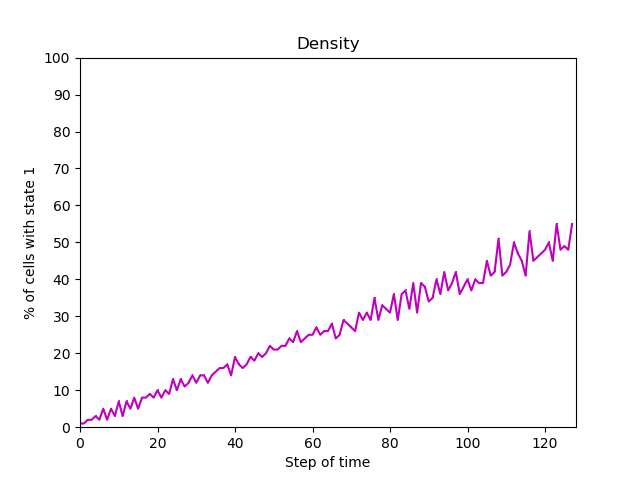
\includegraphics[max width=200mm ,max height=200mm , keepaspectratio ]{SimDensity.png} 
       \caption{Densidad de \rule} 
    \end{figure} 
  \end{subsection} 
  \begin{subsection}{Entropía} 
    \begin{figure}[H] 
    \centering 
    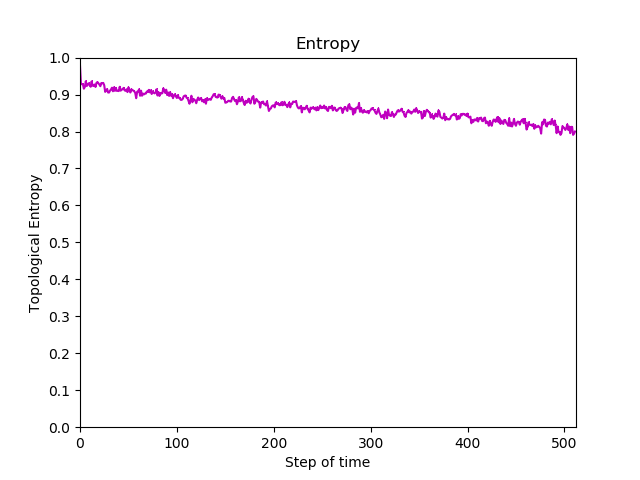
\includegraphics[max width=200mm ,max height=200 mm , keepaspectratio ]{SimEntropy.png} 
    \caption{Entropía de \rule} 
    \end{figure} 
    \end{subsection}
    \begin{subsection}{Exponentes de Lyapunov} 
    \begin{figure}[H] 
    \centering 
    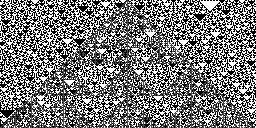
\includegraphics[max width=200mm ,max height=200 mm , keepaspectratio ]{SimDefects.png} 
    \caption{Simulación de los defectos del Exponentes de Lyapunov \rule} 
    \end{figure} 
    \end{subsection} 
    \begin{table}[H] 
    \centering 
    \begin{tabular}{cc} 
    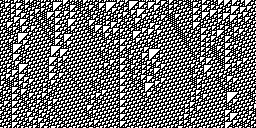
\includegraphics[width=70mm ,max height=70 mm , keepaspectratio]{SimAnalysis.png} & 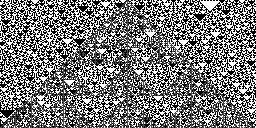
\includegraphics[width=70mm ,max height=70 mm , keepaspectratio]{SimDefects.png} \ 
    \end{tabular} 
    \caption{Simulación de la evolución original contra los defectos del Exponentes de Lyapunov \rule} 
    \end{table} 
    \begin{table}[H] 
    \centering 
    \begin{tabular}{cc} 
    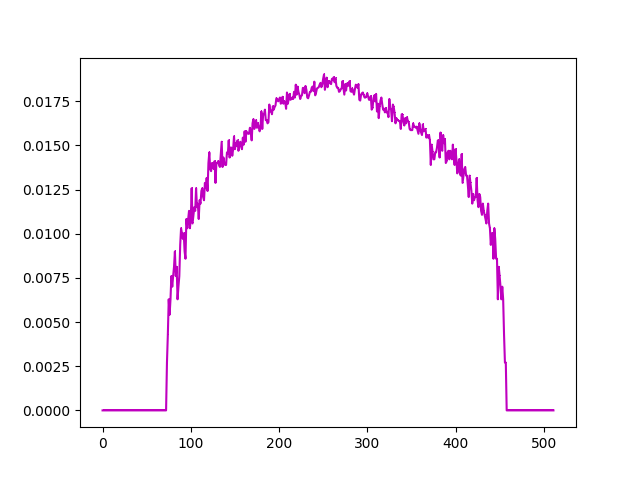
\includegraphics[width=90mm ,max height=90mm , keepaspectratio]{LyapunovExp.png} & 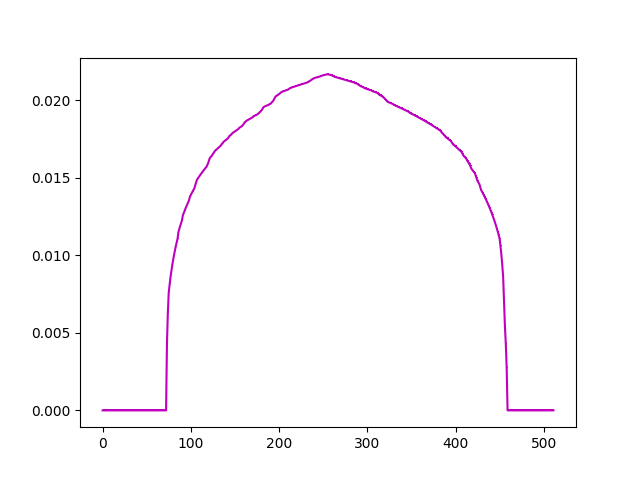
\includegraphics[width=90mm ,max height=90mm , keepaspectratio]{LyapunovExpNorm.png} \ 
    \end{tabular} 
    \caption{Simulación original contra los defectos del Exponentes de Lyapunov \rule} 
    \end{table} 
    \end{section} 
    \clearpage 
  \begin{section}{Análisis Genotípico} 
  \begin{subsection}{Teorìa del Campo Promedio}
  \begin{figure}[H]
  \centering
  \includegraphics[max width=200mm ,max height=200 mm , keepaspectratio ]{../img/MeanField/Plot\r.png}
  \caption{Gráfica del polinomio del campo promedio \rule  }
  \end{figure}
  \begin{table}[H]
  \centering
  \begin{tabular}{|c|c|c|c|}
  \hline Regla & Polinomio  & Punto fijo &Derivada \\ 
  \hline $\r$ & $3*(1 - x)^2*x$  &  $0.42265$  & $0.04639298528584379$ \\  \hline 
  \end{tabular}
  \caption{Datos de la gráfica del campo promedio}
  \end{table}
  \end{subsection}
  \clearpage
  \clearpage
  \begin{subsection}{Campos de atractores}
  \begin{center}
    \begin{longtable}{|c|c|c|c||c|c||c|}
  \hline 
  Num & Ciclo & Altura &Nodos &  Atractor &  Jardin del edén  & Entropia \\ \endhead 
  \hline \hline    1 & 1 & 42 & 11721 & 0 : 0000000000000000   & 38145 : 1001010100000001  & 1.869437 \\ \hline 
  \hline \hline    2 & 14 & 12 & 550 & 3 : 0000000000000011   & 10816 : 0010101001000000  & 2.169767 \\ \hline 
  \hline \hline    3 & 12 & 29 & 1510 & 5 : 0000000000000101   & 40024 : 1001110001011000  & 1.938045 \\ \hline 
  \hline \hline    4 & 12 & 11 & 98 & 32784 : 1000000000010000   & 21813 : 0101010100110101  & 1.823365 \\ \hline 
  \hline \hline    5 & 6 & 5 & 28 & 33153 : 1000000110000001   & 39333 : 1001100110100101  & 1.921185 \\ \hline 
  \hline \hline    6 & 4 & 3 & 16 & 1285 : 0000010100000101   & 29298 : 0111001001110010  & 1.405639 \\ \hline 
  \hline \hline    7 & 2 & 1 & 2 & 13107 : 0011001100110011   & 13107 : 0011001100110011  & -0.0 \\ \hline 
  \hline \hline    8 & 1 & 1 & 1 & 21845 : 0101010101010101   & 21845 : 0101010101010101  & -0.0 \\ \hline 
  \end{longtable} 
  \end{center} 
  \clearpage 
  \begin{longtable}{|c|} 
  \hline 
  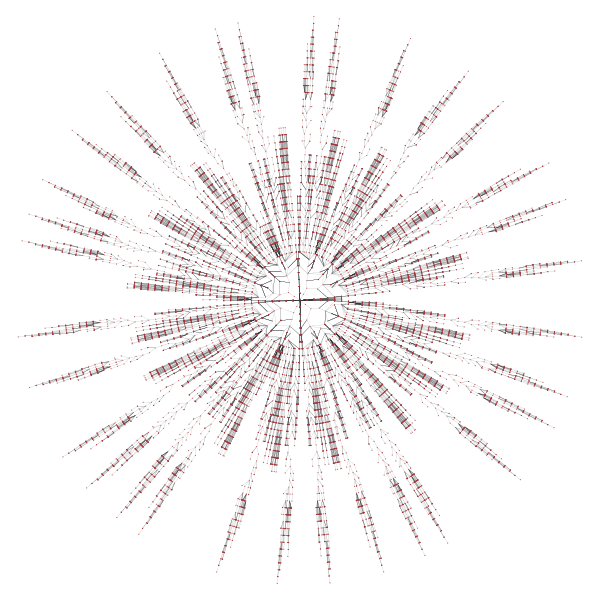
\includegraphics[width=.5\textwidth ,keepaspectratio ]{22_16_s_t_11721s_r_1m_l_42atractor_0_.png} \\ 
    1 \\ \hline 
  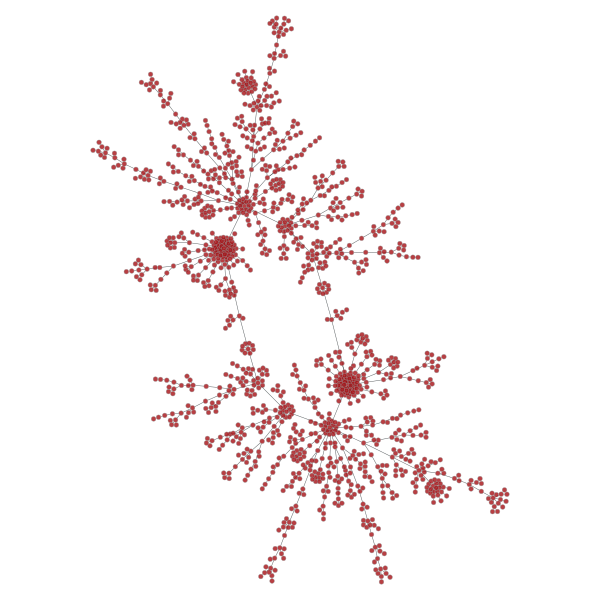
\includegraphics[width=.5\textwidth ,keepaspectratio ]{22_16_s_t_550s_r_14m_l_12atractor_3_.png} \\ 
    2 \\ \hline 
  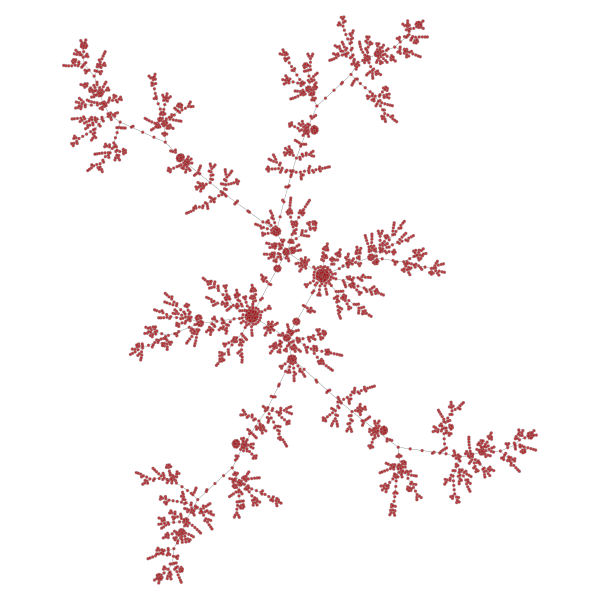
\includegraphics[width=.5\textwidth ,keepaspectratio ]{22_16_s_t_1510s_r_12m_l_29atractor_5_.png} \\ 
    3 \\ \hline 
  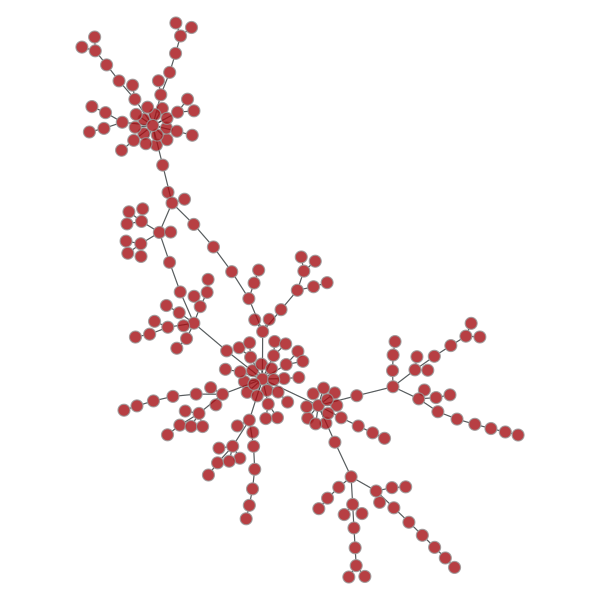
\includegraphics[width=.5\textwidth ,keepaspectratio ]{22_16_s_t_98s_r_12m_l_11atractor_32784_.png} \\ 
    4 \\ \hline 
  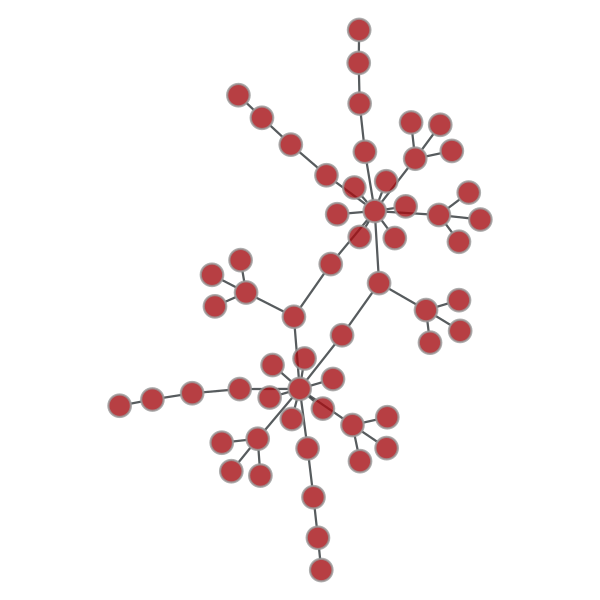
\includegraphics[width=.5\textwidth ,keepaspectratio ]{22_16_s_t_28s_r_6m_l_5atractor_33153_.png} \\ 
    5 \\ \hline 
  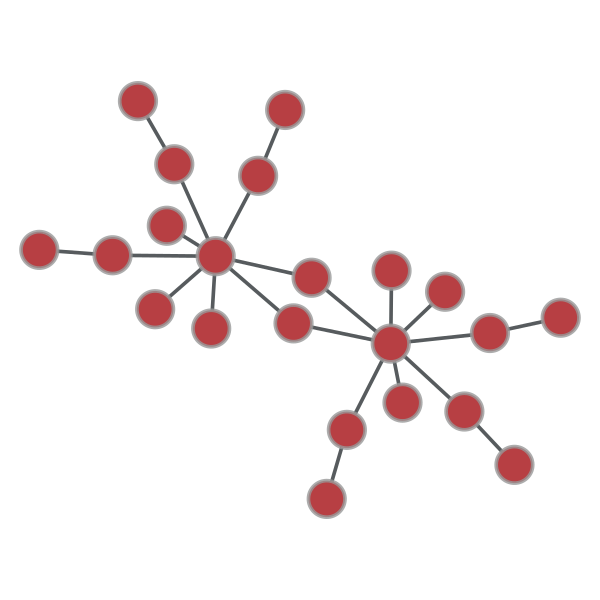
\includegraphics[width=.5\textwidth ,keepaspectratio ]{22_16_s_t_16s_r_4m_l_3atractor_1285_.png} \\ 
    6 \\ \hline 
  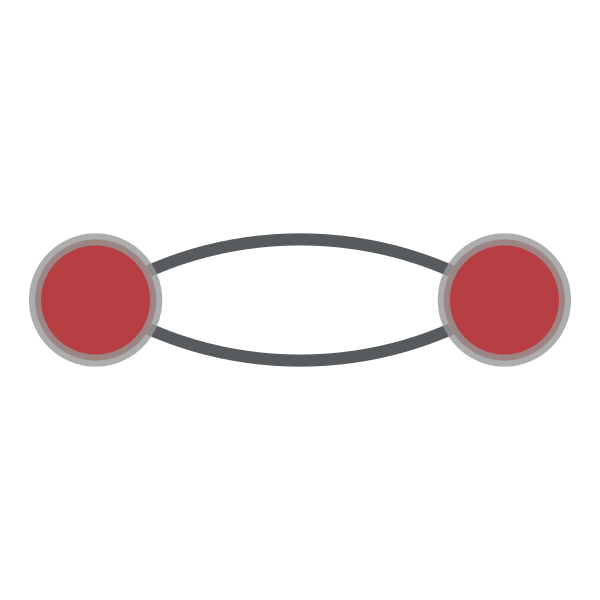
\includegraphics[width=.5\textwidth ,keepaspectratio ]{22_16_s_t_2s_r_2m_l_1atractor_13107_.png} \\ 
    7 \\ \hline 
  
\includegraphics[width=.5\textwidth ,keepaspectratio ]{22_16_s_t_1s_r_1m_l_1atractor_21845_.png} \\ 
    8 \\ \hline 
  \end{longtable}
  \end{subsection} 
 \end{section} 
\end{document}